\section{Выводы}

	Получив результаты изложенные выше в таблицах \ref{projectt1}-\ref{projectt4}, можно рассмотреть целесообразность
		разработки интеллектуальной системы управления. Сравнительный анализ показал, что среднее время ожидания
		человеком значительно меньше, чем у более тривиального решения. Также результаты можно сравнить с помощью
		диаграммы на рисунке \ref{pt1}, где отчётливо видно, что продвинутое программное решение является более эффективном.

	\begin{figure}[h]
		\centering
		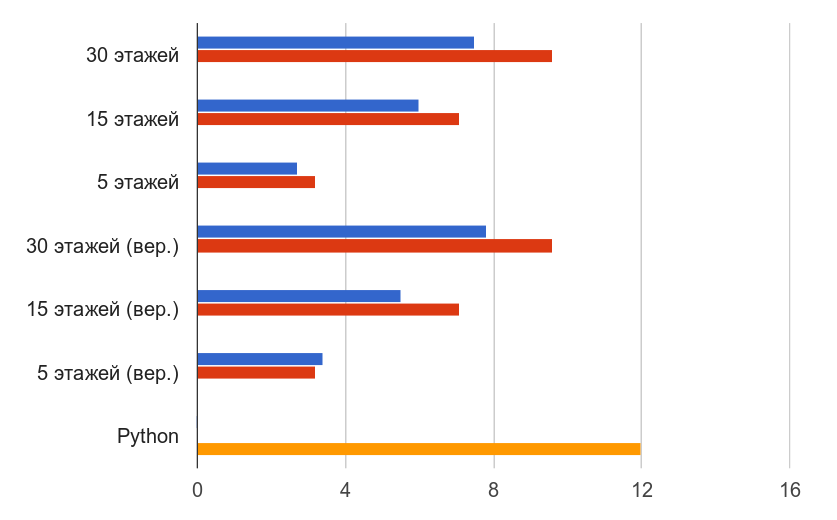
\includegraphics[width=180mm]{src/pictures/projectp1.png}
		\caption{Сравнение по среднему времени ожидания}\label{pt1}
	\end{figure}

	Более того, продвинутое решение требует небольшого улучшения, которое позволит с лёгкостью пройти тест на
		небольшом количестве этажей. Улучшение будет собой представлять не большое правило, которое бы могло увеличить
		глубину обхода дерева вариантов решений.
		
	Но не стоит забывать, что чем сложнее требуемый логический вывод, тем больше ресурсов необходимо системе для
		функционирования. Поэтому необходимо обратить внимание на диаграмму, которая представлена на рисунке \ref{pt2}.

	\begin{figure}[h]
		\centering
		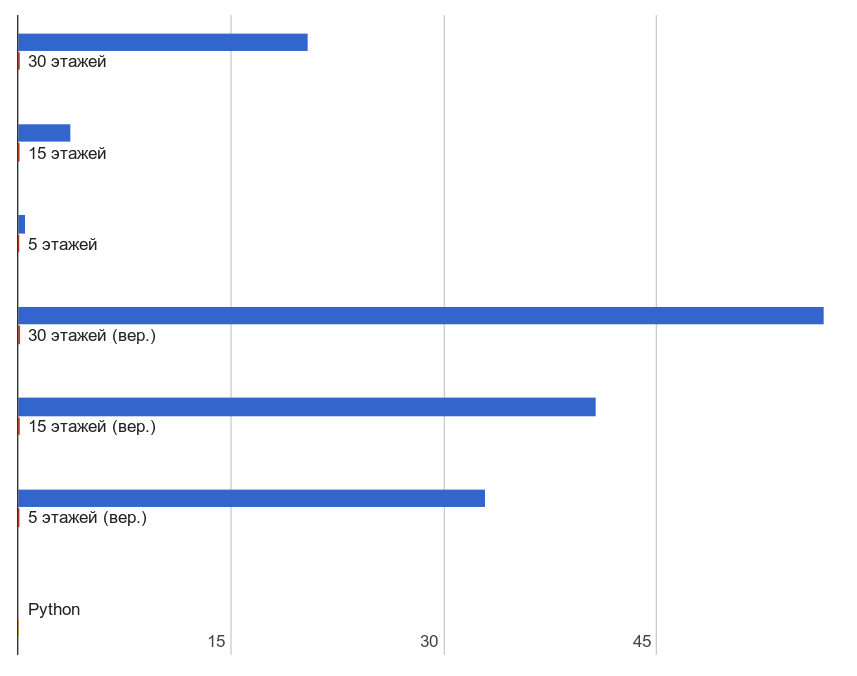
\includegraphics[width=180mm]{src/pictures/projectp2.png}
		\caption{Сравнение по времени выполнения}\label{pt2}
	\end{figure}

	Из диаграммы видно, что время, которое затрачено на построение логического вывода достаточно велико.
		Это показывает, что для своевременного решения необходимо достаточно большое количество ресурсов.
		Несмотря на тот факт, что на стройка разработанного программного обеспечения не будет занимать
		длительное время, что делает продукт более дешёвым, поддержание данной системы становится
		дорогостоящим процессом, за счёт потребности в дорогостоящем оборудовании.

	Исходя из этого имеется необходимость заняться оптимизацией данного программного решения,
		которое позволит снизить потребность в большом объёме ресурсов.

	И тем не менее, в наше время высокопроизводительное оборудование быстро удешевляется, развивается и
		становится более доступным. Более того, для мест со сложной инфраструктурой затраты на
		разработанное программное решение будет вполне целесообразным.

	Важно подчеркнуть ещё тот, что данное программная реализация является решением двух задач: моделирование 
		среды и построение логического вывода. А это значит, что если выделить блок отвечающий
		за моделирование среды и реализовать его на оптимизированном движке, то сразу будет
		получен большой прирост прирост в производительности.

	Таким образом, разработав данное программное решение, была получена платформа для разработки
		новых программных решений. Где можно будет выделить у данной системы два блока, с которыми
		будет возможно вести независимую разработку. Это позволит ускорить процесс развития данной системы
		и появится возможность заменять эти блоки на более сложные решения.
